\chapter{実験}
 実験は,提案された方法の有効性を確保するために実施した. 実験では,図14に示すように,ZMP Inc.が作成した1:10スケールの車両モデルであるRoboCar 1/10を使用した.このモデルには速度コントローラーが含まれ,車両システムの入力は速度のみである. そのため,MPCから取得した速度値を入力に使用し,駆動力フィードバックの代わりに車両速度フィードバックを実装した. 実験のブロック図を図15に示す.表4で実験のセットアップを示す.
\begin{figure}[H]
    \centering
    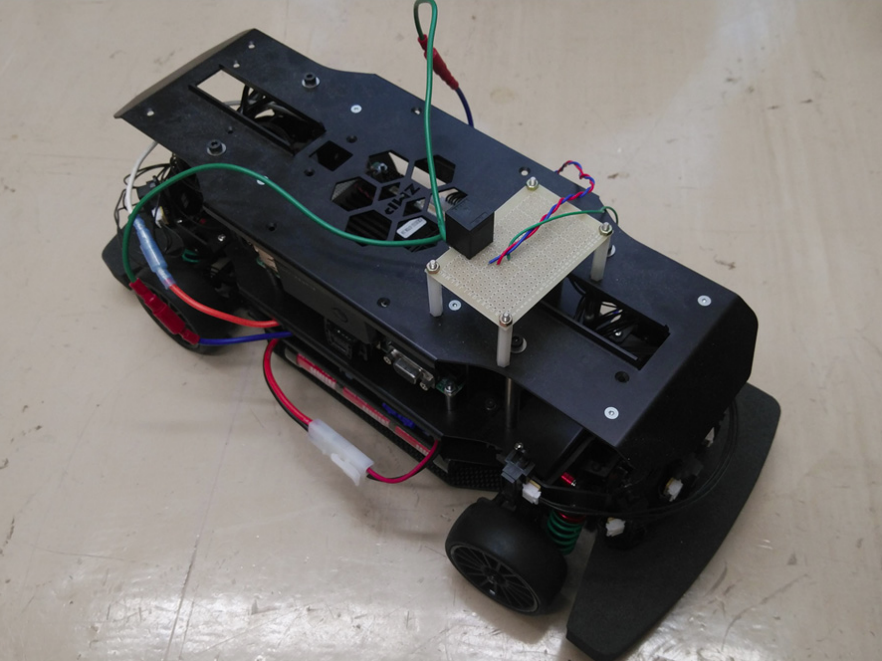
\includegraphics[width=8cm]{./fig/fig14.png}
    \caption{実験車両}
\end{figure}
\begin{figure}[H]
    \centering
    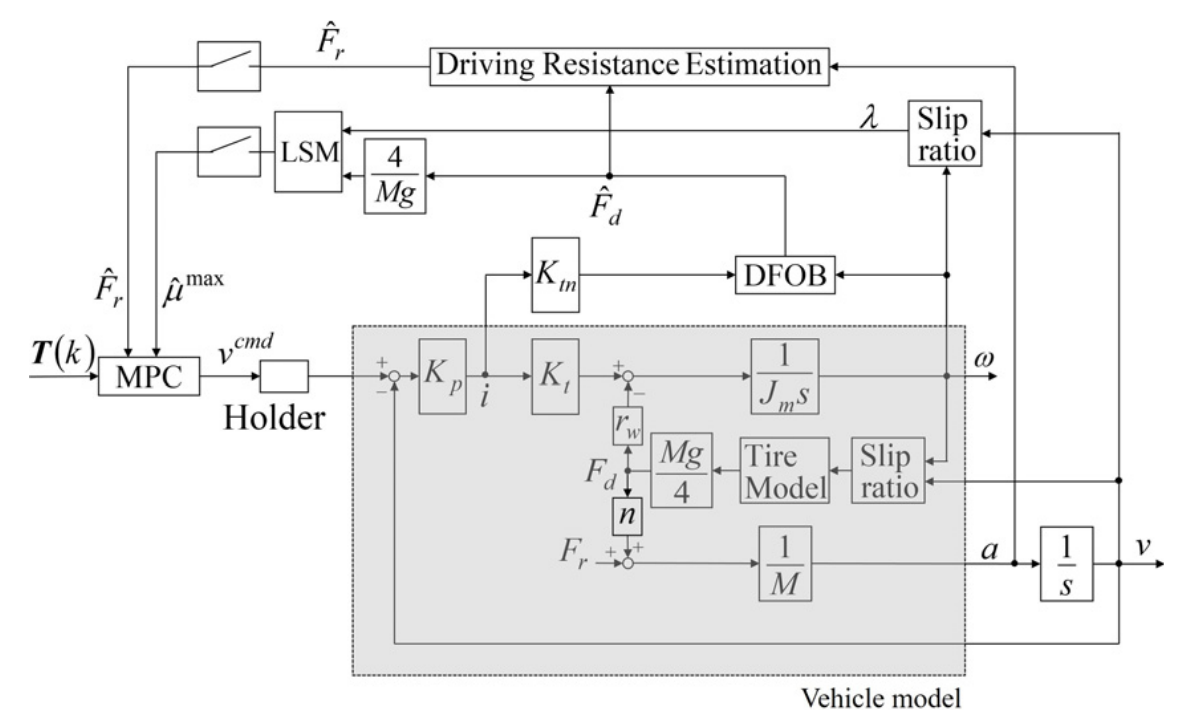
\includegraphics[width=8cm]{./fig/fig15.png}
    \caption{実験のブロック図}
\end{figure}

\begin{table}[htbp]
    \centering
    \caption{実験のパラメータ}
    \scalebox{0.81} {
        \begin{tabular}{|c|c|c|}
            \hline
            Parameter                                 & Value        & Unit      \\ \hline
            Vehicle mass $M$                          & 2.9          & kg        \\ \hline
            Number of controlled wheels $n$           & 2            &           \\ \hline
            Sample time in MPC $T_s$                  & 0.1          & sec       \\ \hline
            Proportional gain $K_p$                   & 50           &           \\ \hline
            prediction horizon $H_p$                  & 30           &           \\ \hline
            Control horizon $H_u$                     & 10           &           \\ \hline
            Safety zone of pedestrian $R_h$           & 0.05         & m         \\ \hline
            Torque coeffcient $K_t$                   & 0.002354     &           \\ \hline
            Motor inertia $J_n$                       & 4.342 x 10 6 & kgm$^2$   \\ \hline
            Motor viscosity coeffcient $D_{\omega h}$ & 9.416 x 10-7 & Nmsec/rad \\ \hline
            Motor coulomb friction $f_{\omega h}$     & 2.532 x 10-3 & Nm        \\ \hline
        \end{tabular}
    }
\end{table}


\begin{figure}[H]
    \centering
    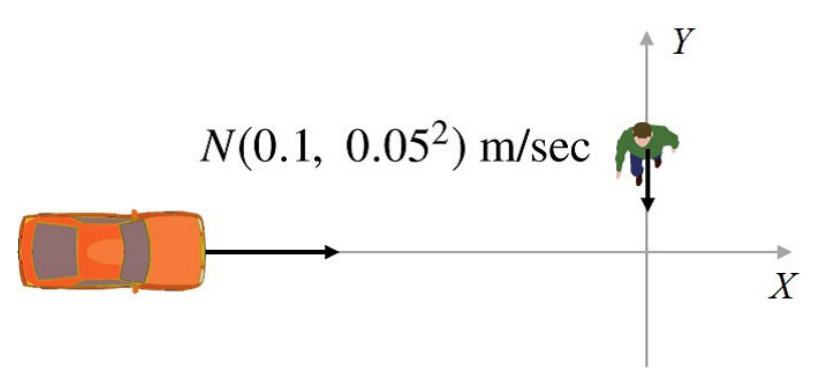
\includegraphics[width=8cm]{./fig/fig16.png}
    \caption{実験の状況}
\end{figure}

実験手順は次のとおり.
\begin{enumerate}
    \item PCで仮想歩行者の位置を生成
    \item PCが情報を車両に送信
    \item 車両は歩行者の位置を受け取り,制御を実行
\end{enumerate}

歩行者の位置は,図16に従ってPCによって計算された.

実験結果を図17,18に示す.図17は,車両と歩行者の位置を示している. 車両は歩行者の前の指令停止地点近くで停止した. それは,提案した方法が衝突回避システムとして非常にうまく機能することを示した. 図18によれば,走行抵抗推定器は定常値に収束する. ただし,シミュレーション結果と比較して,駆動抵抗は駆動力よりもはるかに大きかった. この現象は,転がり抵抗が大きいタイヤが原因で発生したため,制動力を適切に制御して,車両を指令停止点で停止させる必要がある. 補償なしのブレーキシステムの場合,ブレーキ力は変動した. その理由は,MPCが外乱と車両の状態を正確に予測できなかったため,運転抵抗がシステムに影響を与えたためである. 以上より,提案手法の有効性は実験により確認された.
\begin{figure}[H]
    \centering
    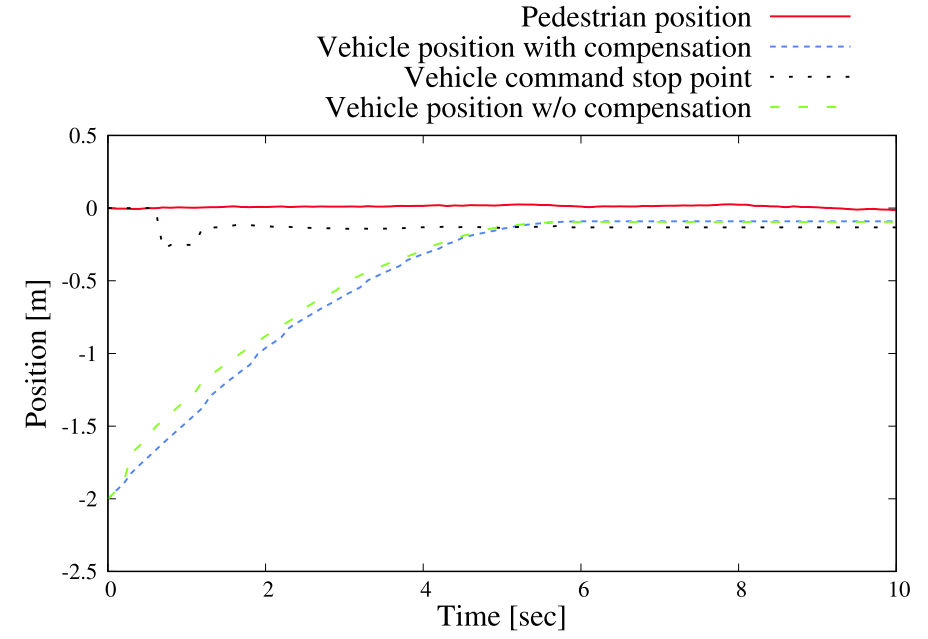
\includegraphics[width=8cm]{./fig/fig17.png}
    \caption{車両位置の実験結果}
\end{figure}
\begin{figure}[H]
    \centering
    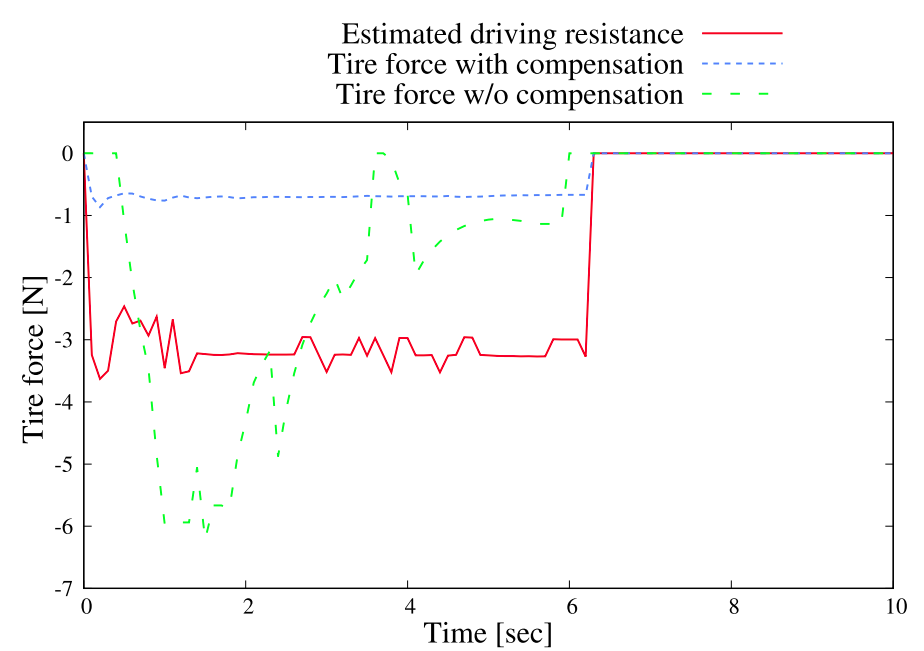
\includegraphics[width=8cm]{./fig/fig18.png}
    \caption{タイヤ力の実験結果}
\end{figure}
